\subsubsection{模型设计}
1、VGG16:SSD网络的基础网络,使用前16层作为特征提取层

2、Conv\{ 4-12 \}:额外添加的层,生成feature map

3、将对conv4的处理抽象成一个类名为L2Norm2d
\begin{uscfigure}
	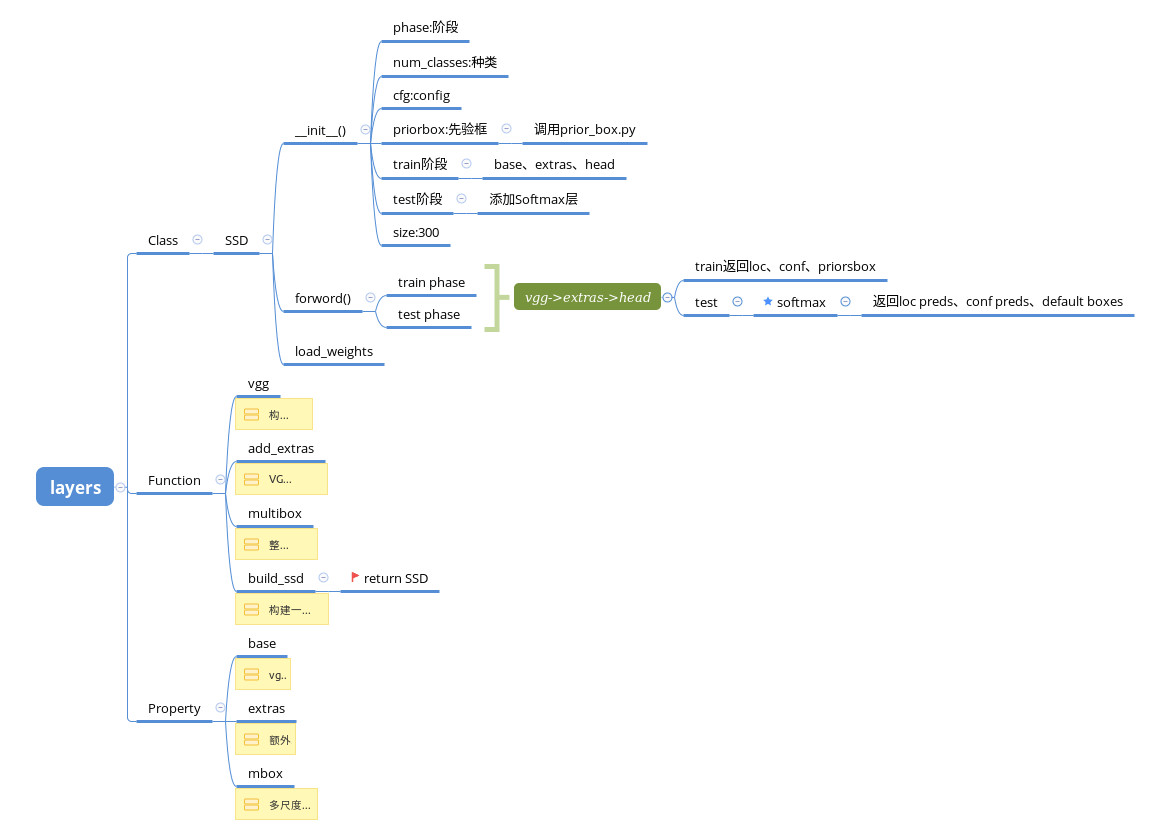
\includegraphics[width=\textwidth]{./Pictures/layers.jpg}	
	\caption{SSD模型设计框架}
\end{uscfigure}
\subsubsection{L2Norm2d}
\begin{lstlisting}[caption={L2Norm2d}]
class L2Norm2d(nn.Module):
	def __init__(self, scale):
		super(L2Norm2d, self).__init__()
		self.scale = scale
		
	def forward(self, x, dim = 1):
		return  self.scale * x *    \
				x.pow(2).sum(dim).  \
				clamp(min=1e-12).	\
				rsqrt().expand_as(x)
\end{lstlisting}
\subsubsection{SSD Layer}
\begin{lstlisting}[caption={SSD layer}]
class SSD300(nn.Module):
	def __init__(self):
		super(SSD300, self).__init__()
	
	#model
	VGG16
	self.conv5(1~3)
	self.conv6
	self.conv7
	self.conv(8~12)(1~2)
\end{lstlisting}

\subsubsection{Multibox Layer}
1、Multibox Layer作为生成Anchor的网络

2、loc\_loss、conf\_loss的计算

\begin{lstlisting}[caption={Multibox layer}]
class MultiBoxLayer(nn.Module):
	num_classes = 2
	num_anchors = [4, 6, 6, 6, 4, 4]
	in_planes = [512, 1024, 512, 256, 256, 256]
	
	for i n range(len(self.in_planes)):
		self.loc_layers.apend(
			nn.Conv2d(self.in_planes[i],
			self.num_anchors[i] * 4,
			kernel_size = 3, padding = 1
			)
		)
		self.conf_layers.apend(
			nn.Conv2d(self.in_planes[i],
			self.num_anchors[i] * 21,
			kernel_size = 3, padding = 1
			)
		)
\end{lstlisting}